This dissertation presents numerous algorithms which aid in identifying safe rooftop landing sites in cities. However, many of our methods are general and can be applied to other domains. In particular, our Polylidar3D algorithm has general applications to any problem domain that requires to polygon extraction from 2D or 3D data. Such problems readily arise in fields such as computational geometry, \ac{GIS}, and robotics. We have released the open-source software implementations of Polylidar3D and its supporting software under the permissive MIT license \cite{saltzer_origin_2020}. I have carefully optimized each software implementation and tested on both Windows and Linux platforms. All software is hosted online using GitHub, a software development and version control hosting website. Our software is currently being used by academic researchers, software engineers, and geographic information system scientists.  The three main software repositories of interest are:

\begin{enumerate}
    \item Polylidar3D - Fast polygon extraction from 2D and 3D data. \\ Hosted at: \url{https://github.com/JeremyBYU/polylidar}
    \item Fast Gaussian Accumulator (FastGA) - Dominant plane normal estimation for 3D scenes. \\  Hosted at: \url{https://github.com/JeremyBYU/FastGaussianAccumulator}
    \item Organized Point Filters (OPF) - Fast smoothing for organized 3D point clouds.
    \\  Hosted at: \url{https://github.com/JeremyBYU/OrganizedPointFilters}
\end{enumerate}

Each software repository is written in C++ for high performance but includes bindings to Python. We utilize CPU parallelism if available. The build system uses \texttt{CMake} and is tested with the \texttt{msbuild} and \texttt{gcc} compilers. Each repository provides documentation through examples as well as the application programming interface (API). Bug reports may be filed at each individual repository. Each section below will provide multi-page screenshots of their respective source code repositories. The screen shot is of the \texttt{README.md} file which provides a brief summary of the software.

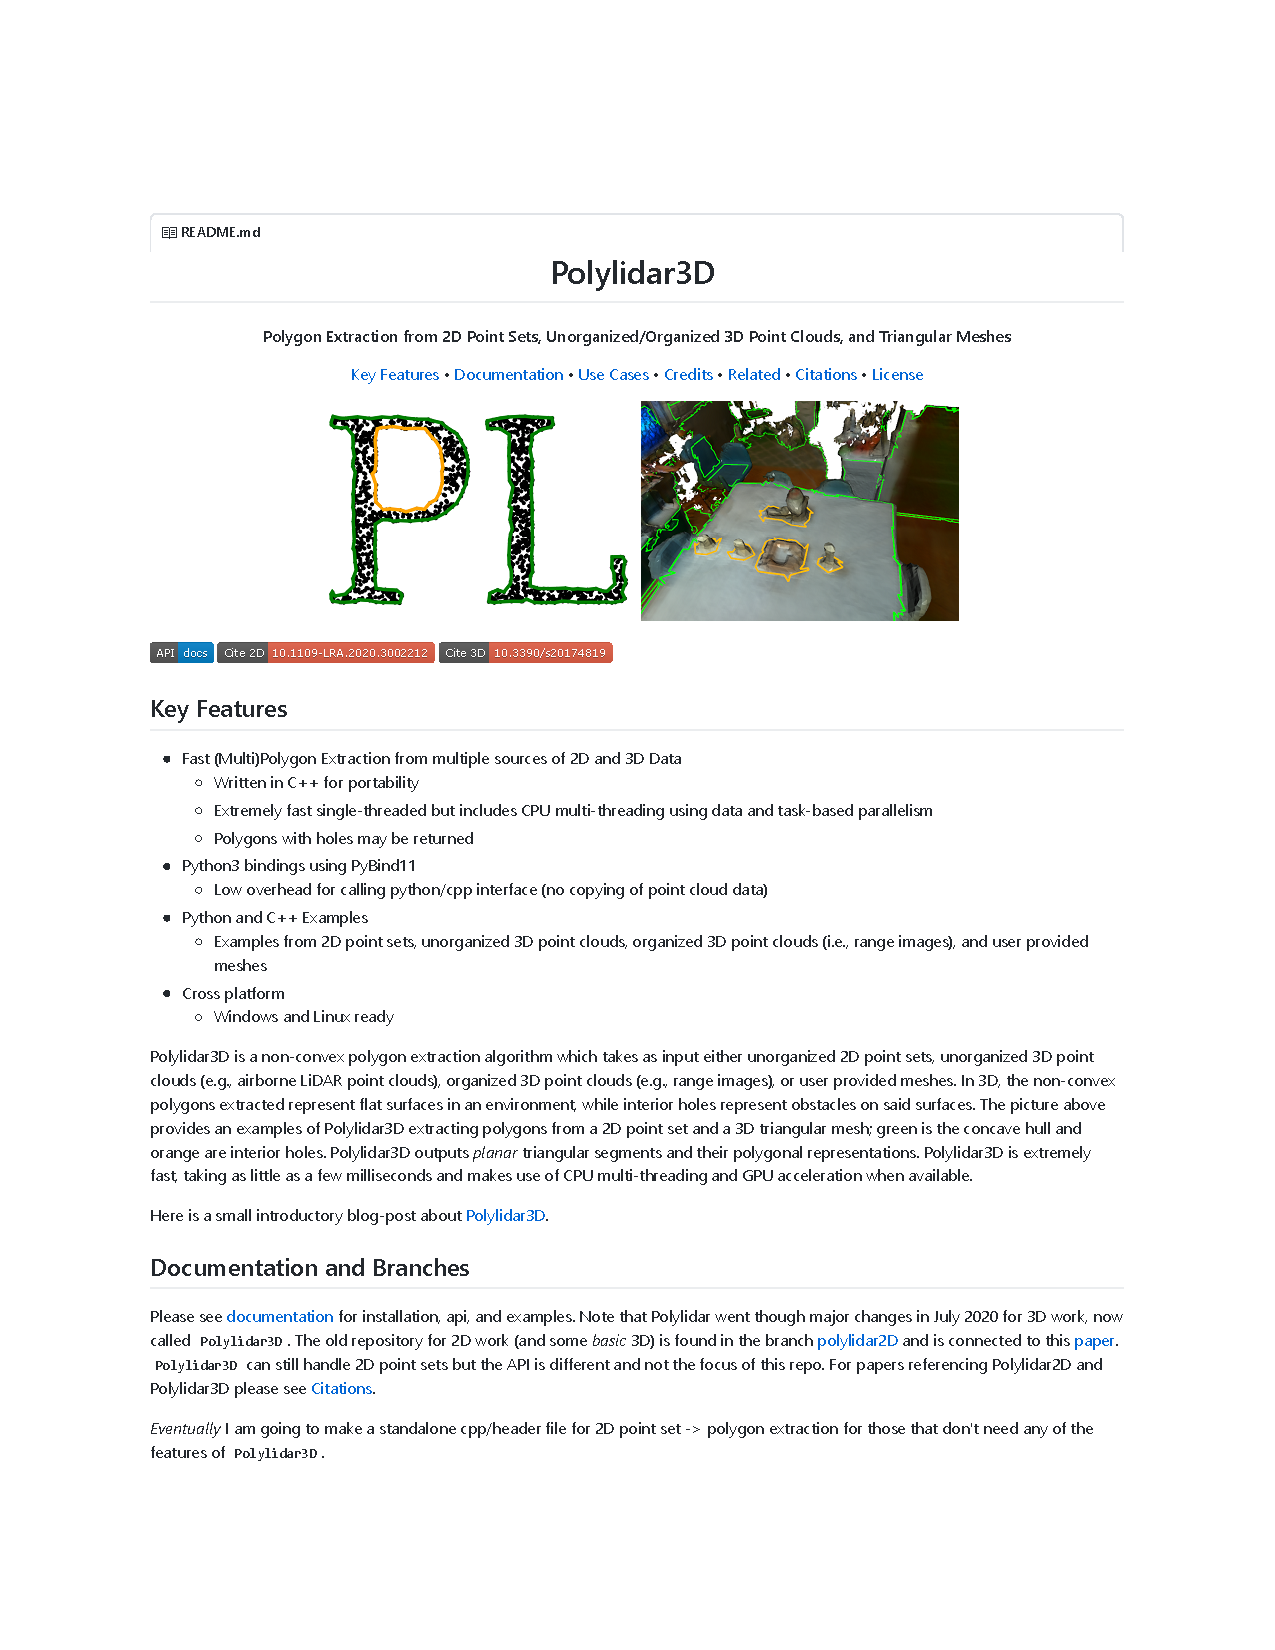
\includepdf[pages=1,pagecommand={\section{Polylidar3D Source Code Summary} Below is a multi-page screenshot of the \texttt{README.md} file for the Polylidar3D source code repository hosted at \url{https://github.com/JeremyBYU/polylidar}. {}}, fitpaper=false, scale=0.95, offset=0 -1.1cm]{appendix_1/imgs/Polylidar3DReadme.pdf}
\includepdf[pages=2-,pagecommand={}, fitpaper=true]{appendix_1/imgs/Polylidar3DReadme.pdf}


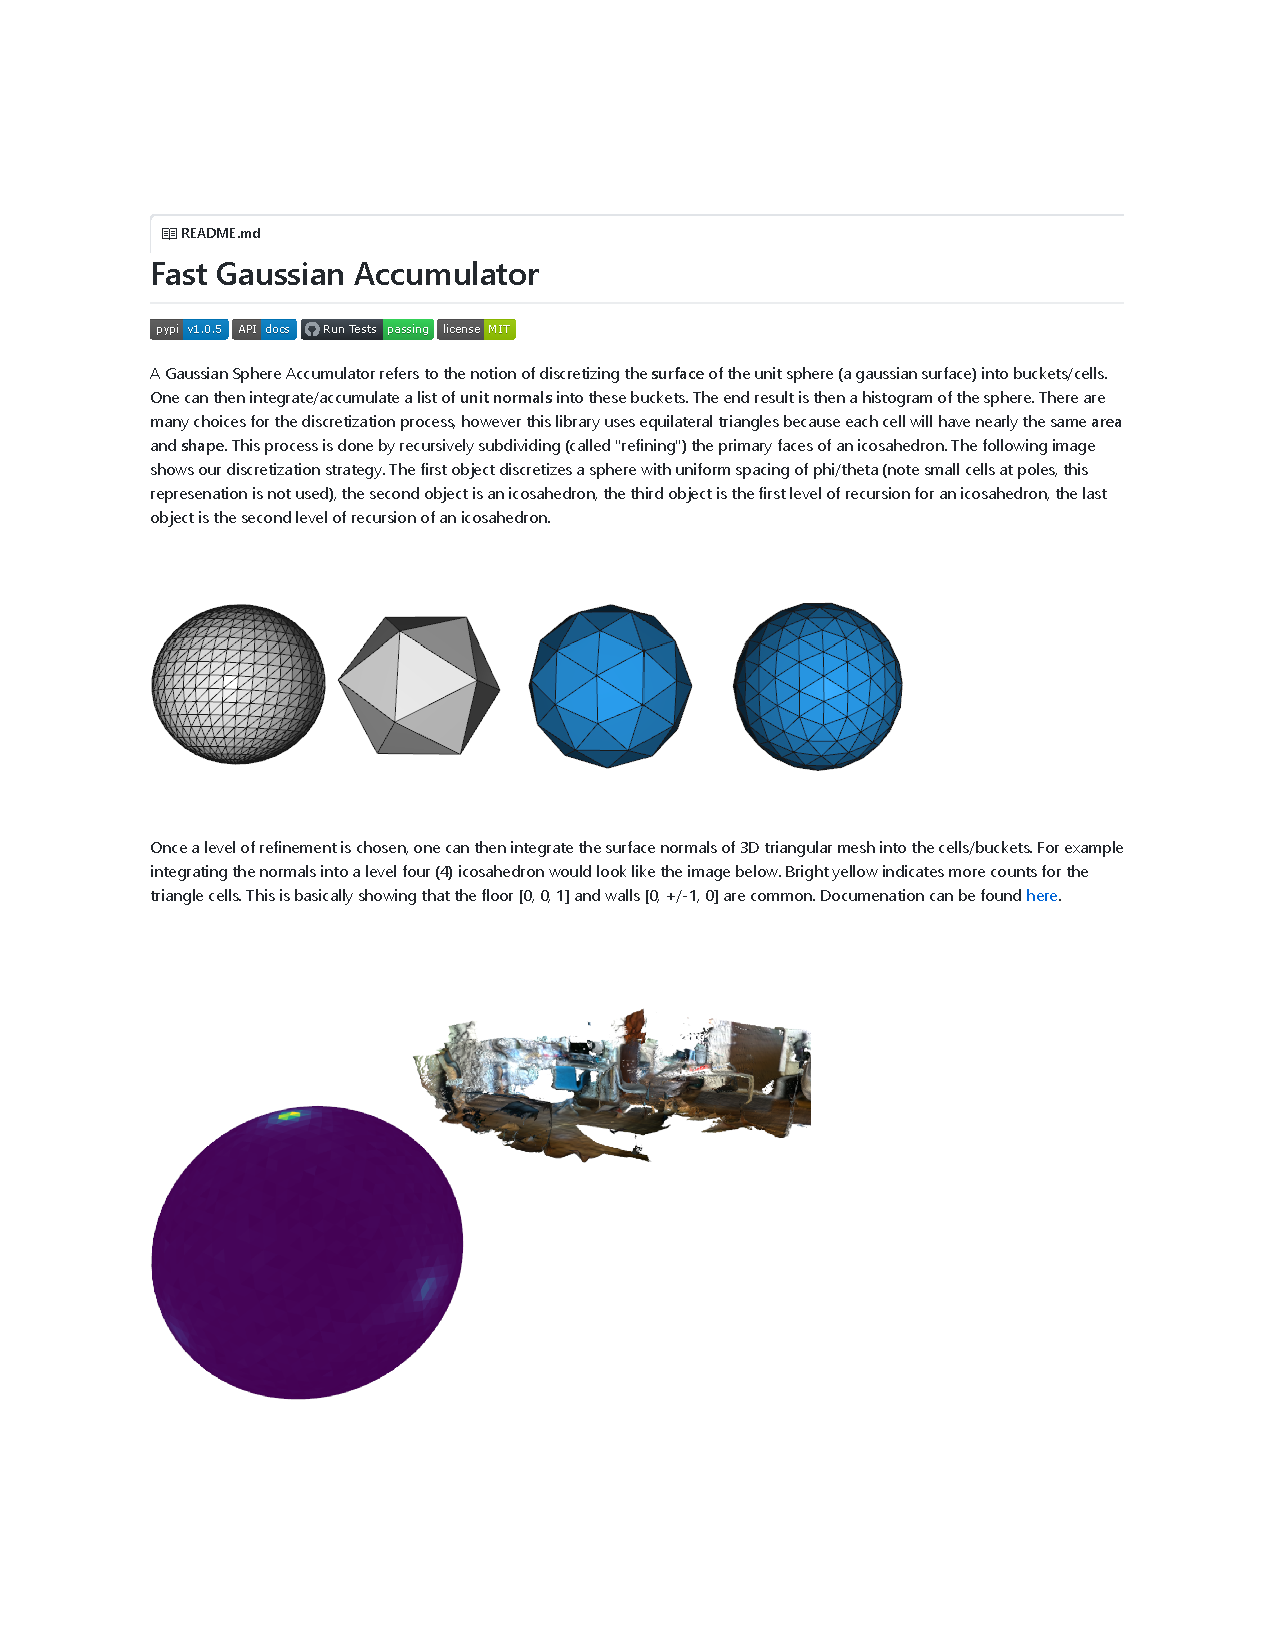
\includepdf[pages=1,pagecommand={\section{Fast Gaussian Accumulator Source Code Summary} Below is a multi-page screenshot of the \texttt{README.md} file for the FastGA source code repository hosted at \url{https://github.com/JeremyBYU/FastGaussianAccumulator}. {}}, fitpaper=false, scale=0.95, offset=0 -1.1cm]{appendix_1/imgs/FastGAReadme.pdf}
\includepdf[pages=2-,pagecommand={}, fitpaper=true]{appendix_1/imgs/FastGAReadme.pdf}


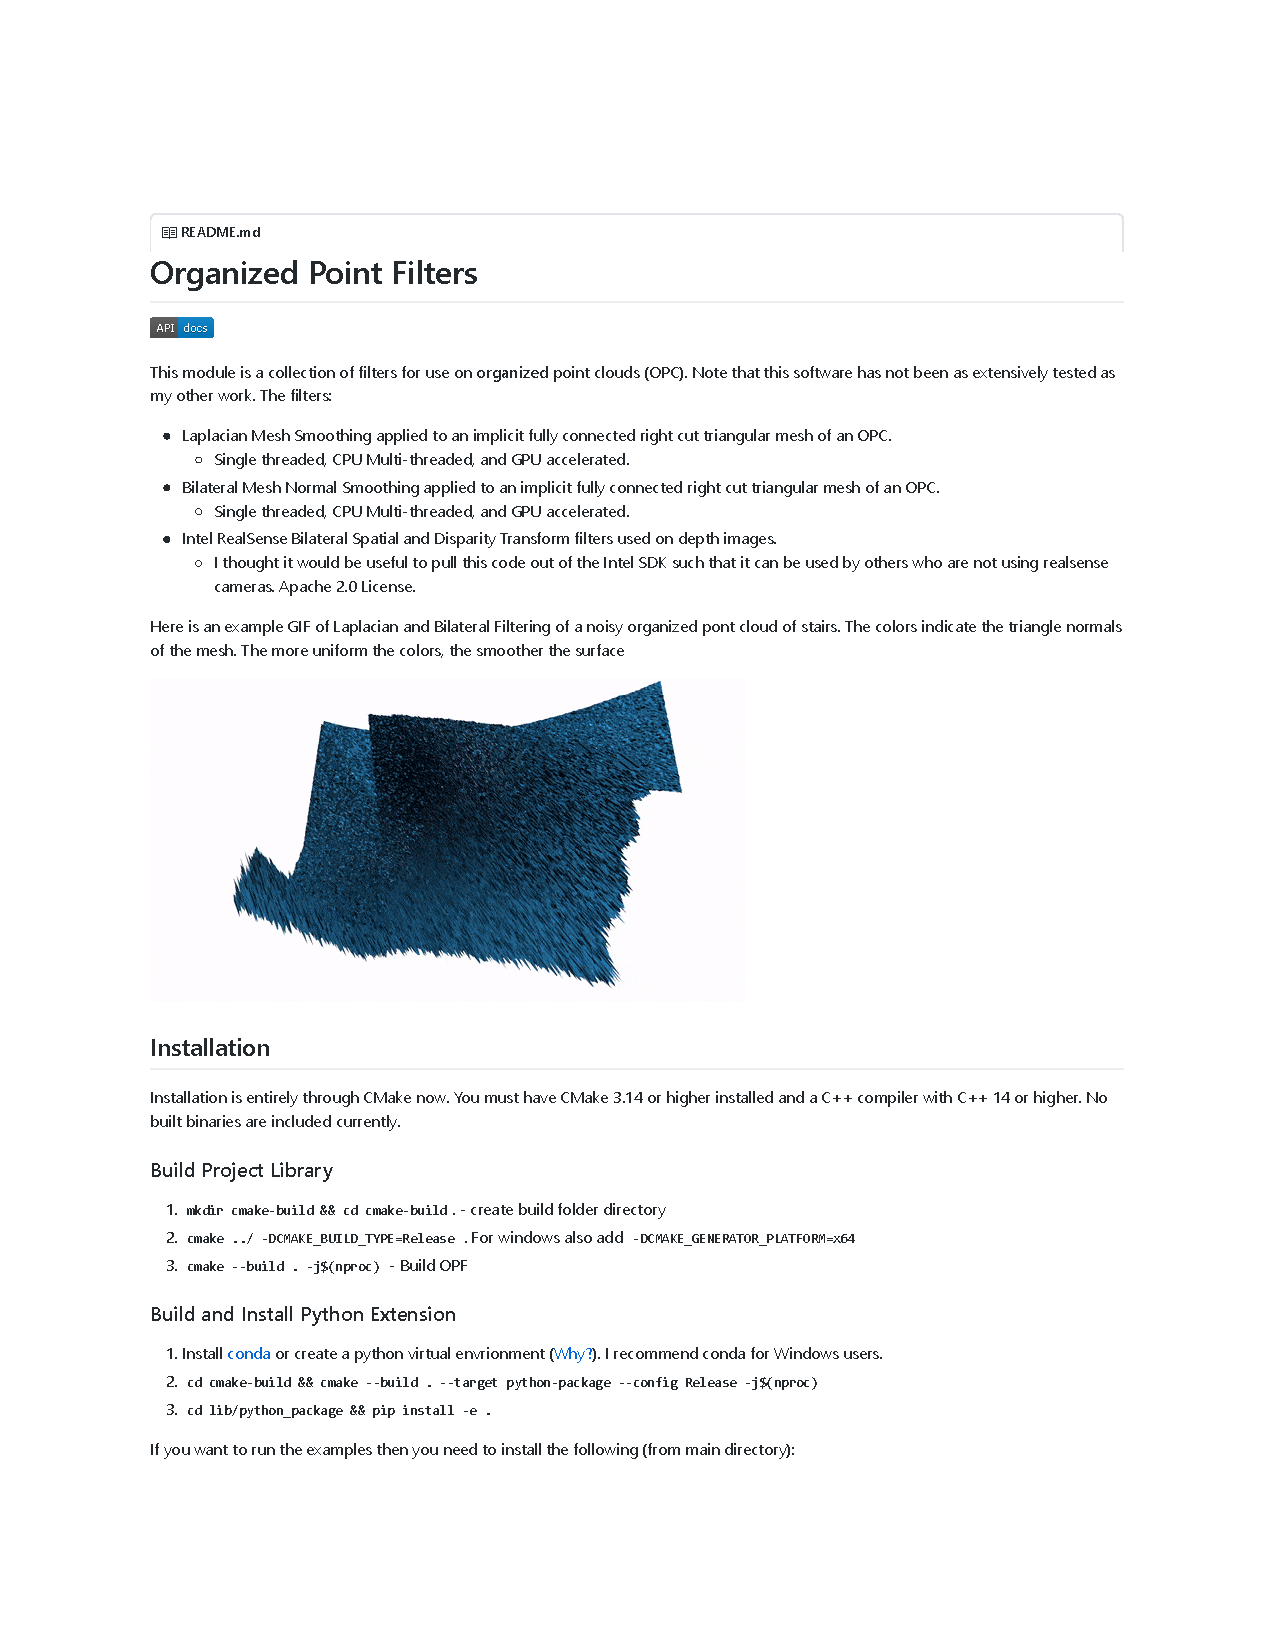
\includepdf[pages=1,pagecommand={\section{Organized Point Filters Source Code Summary} Below is a multi-page screenshot of the \texttt{README.md} file for the OPF source code repository hosted at \url{https://github.com/JeremyBYU/OrganizedPointFilters}. {}}, fitpaper=false, scale=0.95, offset=0 -1.1cm]{appendix_1/imgs/OPFReadme.pdf}
\includepdf[pages=2,pagecommand={}, fitpaper=true]{appendix_1/imgs/OPFReadme.pdf}


